\chapter{Securing the network infrastructure}

\section{Securing device access}

\subsection{Edge router}

There are many approaches to secure the edge router:

\begin{itemize}
\item \textbf{Single router approach:}  a single router connects internal LAN to the Internet.  All security policies are configured on this device. This is commonly deployed in small networks such as branch and small office, SOHO sites. The required security features can be supported by ISRs.

\item \textbf{Defense-in-depth approach:} there are three primary layers of defense: the edge router, the firewall, and an internal router that connects to the protected LAN (Figure \ref{DefInDepth}). The edge router first screens the traffic before forwarding to the dedicated firewall appliance. The firewall provides additional access control by tracking the state of the connections. By default, the firewall denies the initiation of connections from the outside (untrusted) networks. 
%However, it allows the internal users to establish connections to the untrusted networks and permits the responses to come back through the firewall. It can also perform user authentication.

\item \textbf{DMZ approach:} A variation of the defense-in-depth approach is the  DMZ approach (Figure \ref{DMZ}). This approach includes an intermediate area, often called the demilitarized zone (DMZ). The firewall is set up to permit the required connections, such as HTTP, from the outside networks to the public servers in the DMZ. The firewall serves as the primary protection for all devices in the DMZ.
\end{itemize}

Three areas of router security must be maintained:

\begin{itemize}
\item \textbf{Physical security:} Place the router and physical devices that connect to it in a secure locked and dedicated room 

\item \textbf{Operating system security:} Configure the router with the maximum amount of memory possible, Use the latest, stable version of the operating system, Keep a secure copy of router operating system images and router configuration files

\item \textbf{Router Hardening:} Secure administrative control, Disable unnecessary ports, interfaces and services
\end{itemize}

\begin{figure}[hbtp]
\caption{Defense-in-depth approach}\label{DefInDepth}
\centering
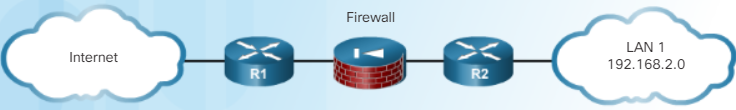
\includegraphics[ scale=0.5 ]{pictures/DefInDepth.PNG}
\end{figure}

\begin{figure}[hbtp]
\caption{DMZ approach}\label{DMZ}
\centering
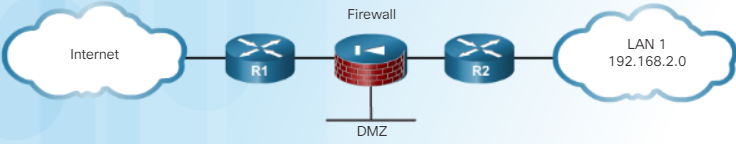
\includegraphics[scale=0.5]{pictures/DMZ.PNG}
\end{figure}

A router can be accessed for administrative purposes locally or remotely. Local access to a router requires a direct connection to a console port, and using a computer that is running terminal emulation software. The most common remote access method involves allowing SSH, HTTPS, or SNMP connections to the router from a computer. Precautions should be taken when accessing the network remotely:

\begin{itemize}
\item Encrypt all traffic between the administrator computer and the router. Use SSH version 2 and HTTPS.
\item Establish a dedicated management network
\item Configure a packet filter to allow only the identified administration hosts and preferred protocols to access the router.
\item Configure and establish a VPN connection to the local network before connecting to a router management interface.
\end{itemize}

\subsection{Administrative access}

\paragraph{Type of management access:} 

When logging and managing information, the information flow between management hosts and the managed devices can take two paths: In-band (SSH, SNMP, etc.) and Out-of-band (OOB, use console port). As a general rule, for security purposes, OOB management is appropriate for large enterprise networks. The OOB management remains unaffected by the downed link. In-band management is recommended in smaller networks as a means of achieving a more cost-effective security deployment. It is made as secure as possible using secure management protocols, for example SSH, IPsec.

\paragraph{Strong password:} 

On Cisco devices, password-leading spaces are ignored but spaces after the first character are not ignored. One method to create a strong password is to use a blank space in the password or create a phrase made of many words. This is called a \emph{passphrase}. A passphrase is often easier to remember than a complex password and more difficult to guess.

\paragraph{Secret Password Algorithms:} 

All passwords in Cisco IOS uses an MD5 hash by default. However, MD5 hashes are no longer considered secure. Therefore, it is now recommended that you configure all passwords using either type 8 \code{sha256} or type 9 \code{scrypt} passwords.

\begin{sexylisting}{Password algorithm type 9 with uncrypted password}
R1(config)# enable algorithm-type scrypt secret cisco12345
R1(config)# username Huy algorithm-type scrypt secret cisco12345
\end{sexylisting}


\subsection{Virtual logins}

The following Cisco IOS login enhancements commands increase the security of virtual login connections.

\begin{sexylisting}{Login security commands}
R1(config)# login block-for 15 attempts 5 within 60
R1(config)# login quite-mode access-class PERMIT-ADMIN
R1(config)# login delay 10
R1(config)# login on-access log
R1(config)# login on-failure log
\end{sexylisting}

The \code{login block-for} command can defend against DoS attacks by disabling logins for 60 seconds if more than 5 login failures occur in 15 seconds or less. Specifically, the login block-for command operates in two modes: Normal mode and Quite mode. When quiet mode is enabled, all login attempts, including valid administrative access, are not permitted. However, this behavior can be overridden using the \code{login quiet-mode} command. This command maps to an ACL that identifies the permitted hosts. \\

The \code{login delay} command specifies a number of seconds the user must wait between unsuccessful login attempts. The \code{login on-success} and \code{login on-failure} commands generate syslog messages for successful and unsuccessful login attempts. The \code{security auth failure rate} command can be configured to generate a log message when the login failure rate is exceeded.\\

Use the \code{show login} command to verify the login block-for command settings and current mode. The \code{show login failures} command displays additional information regarding the failed attempts, such as the IP address from which the failed login attempts originated.\\

These login enhancements do \emph{not} apply to console connections. When dealing with console connections, it is assumed that only authorized personnel have physical access to the devices.\\

\note These login enhancements can only be enabled if the local database is used for authentication for local and remote access. If the lines are configured for password authentication only, then the enhanced login features are not enabled.

\subsection{Configuring SSH}

There are four requirements the router must meet before configuring SSH:

\begin{itemize}
\item Runs a Cisco IOS release that supports SSH
\item Uses a unique hostname
\item Contains the correct domain name of the network
\item Configured for local authentication or AAA services
\end{itemize}

The five steps needed to configure a Cisco router to support SSH with local authentication:

\begin{enumerate}
\item Configure the IP domain name of the network
\item Create RSA key to encrypt the SSH traffic
\item Ensure that there is a valid local database username entry.
\item Enable vty inbound SSH sessions using the line vty commands
\item Verify SSH and display the generated keys
\end{enumerate}

\begin{sexylisting}{Configuring SSH}
R1(config)# ip domain-name cisco.com

R1(config)# crypto key zeroize rsa
R1(config)# crypto key generate rsa general-keys modulus 1024

R1(config)# ip ssh version 2
R1(config)# username Huy algorithm-type scrypt secret cisco12345

R1(config)# line vty 0 4
R1(config)# login local
R1(config)# transport input ssh

R1(config)# ip ssh time-out 90
R1(config)# ip ssh authentication-retries 2

R1# sh crypto key mypubkey rsa
R1# sh ssh
\end{sexylisting}

If there are existing key pairs, it is recommended that they are removed using the \code{crypto key zeroize rsa} command. To verify the status of the client connections, use the \code{sh ssh} command. The default SSH timeouts and authentication parameters can be altered using \code{ip ssh time-out} and \code{ip ssh authentication-retries} commands.

\section{Administrative roles}

Cisco IOS software has two methods of providing infrastructure access: privilege level and role-based CLI. Both methods help determine who should be allowed to connect to the device and what that person should be able to do with it. Role-based CLI access provides more granularity and control.

\subsection{Privilege levels}

By default, the Cisco IOS software CLI has two levels of access to commands:

\begin{itemize}
\item \textbf{Level 1:} User EXEC mode -- The lowest user privileges and allows only user-level commands available at the \verb|router>| prompt.
\item \textbf{Level 15:} Privileged EXEC mode -- the user has full access to view and change the configuration, including viewing the running the configuration.
\end{itemize}

The first command shown below configures privilege level 5, so that any level-5 user has access to all the commands available for the level 1 to 4 and the \texttt{ping} command. Remember that not all commands are available for privilege level 5. For example, level-5 users cannot reload the router. To enable access to the reload command, use the command \code{privilege exec level 5 reload}. The second command assigns a privilege level to a specific EXEC mode password. The last assigns privilege level \texttt{5} to user \texttt{SUPPORT}. 

\begin{sexylisting}{Privilege level configuration}
R1(config)# privilege exec level 5 ping 
R1(config)# enable algorithm-type scrypt secret level 5 cisco5
R1(config)# username SUPPORT privilege 5 algorithm-type scrypt secret cisco5
\end{sexylisting}

The use of privilege levels has its limitations:

\begin{itemize}
\item No access control to specific interfaces, ports, logical interfaces, and slots on a router.
\item Commands available at lower privilege levels are always executable at higher levels.
\item Commands specifically set at a higher privilege level are not available for lower privileged users.
\item Assigning a command with multiple keywords allows access to all commands that use those keywords. For example, allowing access to show ip route allows the user access to all show and show ip commands.
\end{itemize}

\subsection{Role-based CLI}

Role-based CLI enhances the security of the device by defining the set of CLI commands accessible by a specific user. Users only see the CLI commands applicable to the ports and CLI to which they have access. Therefore, the router appears to be less complex, and commands are easier to identify when using the help feature on the device.\\

Role-based CLI provides three types of views that dictate which commands are available:

\begin{itemize}
\item \textbf{Root view:} Only a root view user can configure a new view and add or remove commands from the existing views.
\item \textbf{CLI view:} A specific set of commands can be bundled into a CLI view.  A view does not inherit commands from any other view. Additionally, the same commands can be used in multiple views.
\item \textbf{Superview:} A superview consists of one or more CLI views. Users who are logged into a superview can access all the commands that are configured for any of the CLI views that are part of the superview. Deleting a superview does not delete the associated CLI views. The CLI views remain available to be assigned to another superview.
\item \note Commands cannot be configured for a superview. An administrator must add commands to the CLI view and add that CLI view to the superview.
\end{itemize}

The following commands show how to create a CLI view:

\begin{sexylisting}{CLI View configuration}
R1(config)# aaa new-model
R1(config)# parser view SUPPORT
R1(config-view)# secret cisco
R1(config-view)# commands exec include show
R1(config-view)# end
R1#
R1# enable view SUPPORT
\end{sexylisting}

In the above example, the \code{commands} command assigns all \code{show} commands to the EXEC mode of the view. To access existing views, enter the \code{enable view view-name} command in user mode and enter the password that was assigned to the custom view. Use the question mark (?) command to verify that the commands available in the view are correct.\\

The following commands show how to create a Superview:

\begin{sexylisting}{Superview configuration}
R1(config)# parser view JR-ADMIN superview
R1(config-view)# secret cisco2
R1(config-view)# view SHOWVIEW
R1(config-view)# view VERIFYVIEW
R1(config-view)# view REBOOTVIEW
R1(config-view)# end
\end{sexylisting}

You must be in root view to configure a superview. To confirm that root view is being used, use either the \code{enable view} or \code{enable view root} command. In the above example, more than one CLI view are assigned to the current superview using \code{view} command. To access the superview, use the \code{enable view} command followed by the name of the superview, and provide the password. Use the question mark (?) command to verify that the commands available in the view are correct.\\

From the root view, use the \code{show parser view all} command to see a summary of all views. Notice how the asterisk identifies superviews.

\section{IOS image and Configuration files}

The \textbf{Cisco IOS resilient configuration} feature maintains a secure working copy of the router IOS image file and a copy of the running configuration file. These secure files cannot be removed by the user and are referred to as the primary bootset.\\

To secure the IOS image and enable Cisco IOS image resilience, use the \code{secure boot-image} command.  The Cisco IOS image resilience feature can only be disabled through a console session using the no form of the command. This command functions properly only when the system is configured to run an image from a flash drive with an ATA interface. Additionally, the running image must be loaded from secured storage. Images that are loaded from a remote location, such as a TFTP server, cannot be secured.\\

To take a snapshot of the router running configuration and securely archive it in persistent storage, use the \code{secure boot-config} global configuration mode command.\\

Secured files do not appear in the output of a dir command that is issued from the CLI. This is because the Cisco IOS file system prevents secure files from being listed. Use the \code{show secure bootset} command to verify the existence of the archive.\\

\textbf{Restore a primary bootset} from a secure archive after the router has been tampered with:

\begin{enumerate}
\item Reload the router using the reload command. If necessary, issue the break sequence to enter ROMmon mode.
\item From ROMmon mode, enter the dir command to list the contents of the device that contains the secure bootset file.
\item Boot the router with the secure bootset image using the boot command followed by the flash memory location (e.g. flash0), a colon, and the filename found in Step 2.
\item Enter global configuration mode and restore the secure configuration to a filename of your choice.
\item Exit global configuration mode and issue the copy command to copy the rescued configuration file to the running configuration.
\end{enumerate}

\begin{sexylisting}{Restore a primary bootset}
Router# reload

rommon 1 > dir flash0:
rommon 2 > boot flash0:c1900-universalk9-mz.SPA.154-3.M2.bin

Router> enable
Router# conf t
Router(config)# secure boot-config restore flash0:rescue-cfg
Router(config)# end
Router# copy flash0:rescue-cfg running-config
\end{sexylisting}

The Cisco IOS Resilient feature provides a  secure and authenticated method for copying router configuration or router image files to a remote location, that is \textbf{Secure Copy Protocol (SCP) feature}. SCP relies on SSH and requires that AAA authentication.  The following commands configure the router for server-side SCP with local AAA:

\begin{sexylisting}{Configure SCP with local AAA}
R1(config)# ip domain-name cisco.com
R1(config)# crypto key generate rsa general-keys modulus 1024
R1(config)# username Huy algorithm-type scrypt secret cisco12345
R1(config)# aaa new-model 
R1(config)# aaa authentication login default local 
R1(config)# aaa authorization exec default local
R1(config)# ip scp server enable
\end{sexylisting}

With the above configuration, R1 is now an SCP server and will use SSH connections to accept secure copy transfers from authenticated and authorized users. Transfers can originate from any SCP client (router, switch, or workstation). \\

For example, you want to transfer a backup file from R2 to R1. On R2, use the copy command. Specify the source file location first \code{flash0:R2backup.cfg} and then the destination \code{scp:}. Answer the series of prompts to establish a connection to the SCP server on R1. On R1, you can enter the \code{debug ip scp} command to watch the transfer proceed.\\

An attacker could gain control of that device through the password recovery procedure. An administrator can mitigate this potential security breach by using the \code{no service password-recovery} global configuration mode command. This command disables all access to ROMmon mode. \\

To recover a device with password-recovery disabled, initiate the break sequence within five seconds after the image decompresses during the boot. You are prompted to confirm the break key action. After the action is confirmed, the startup configuration is completely erased, the router boots with the factory default configuration, and therefore, the password recovery procedure is enabled. If you do not confirm the break action, the router boots normally with the no service password-recovery command enabled.\\



\section{Syslog}

\subsection{Introduction}

The syslog protocol allows networking devices to send their system messages across the network to syslog servers. The syslog server serves as an event message collector. Syslog messages are sent using \textbf{UDP} port \textbf{514}. The syslog logging service provides three primary functions:

\begin{itemize}
\item Gather logging information
\item Select the type of logging information
\item Specify the destination of captured syslog messages
\end{itemize}

Syslog messages may be sent to an internal buffer. Messages sent to the internal buffer (RAM) are only viewable through the CLI of the device (console line, terminal line). Alternatively, syslog messages may be sent across the network to an external syslog server.\\

To view syslog messages, a syslog server must be installed on a workstation. One advantage of viewing syslog messages on a syslog server is the ability to perform granular searches through the data. Also, a network administrator can quickly delete unimportant syslog messages from the database.

\subsection{Severity level and Facility}
Cisco devices produce syslog messages as a result of network events. Every syslog message contains a \textbf{severity level} and a \textbf{facility}. The security level can be shown as a number. The smaller the number, the more critical syslog alarms (Table \ref{tab:Syslog}).\\

\begin{table}[hbtp]
\centering\caption{Syslog Severity level}\label{tab:Syslog}
\begin{tabular}{|c|c| p{10cm}| }
\hline
\head{Severity level} & \head{Name} & \head{Explanation}\\
\hline 
0 & Emergency & A "panic" condition, System unusable \\\hline 
1 & Alert & Should be corrected immediately, e.g. loss of backup ISP connection \\\hline 
2 & Critical & Critical condition \\\hline 
3 & Error & Error condition, Non-urgent failures \\\hline 
4 & Warning & NOT an error, but indication that an error will occur if action is not taken, e.g. file system 85\% full \\\hline 
5 & Notification & Normal but significant condition \\\hline 
6 & Informational & Not affect functionality, harvested for reporting, measuring throughput,\\\hline 
7 & Debugging & Debugging message \\
\hline
\end{tabular}
\end{table}

Level 0 -- 4 are error messages. Level 5 notifies system messages such as interface up or down transitions and system restart messages. Level 6 generates messages , for example, when the device is booting. By default, Cisco routers and switches send log messages up to level 6 of severity (levels 0 through 6) to the console.

\subsection{Message format}

By default, the format of syslog messages on the Cisco IOS Software is as follows:

\begin{verbatim}
seq no: timestamp: %facility-severity-MNEMONIC: description
00:00:46: %LINK-3-UPDOWN: Interface Port-channel1, changed state to up
\end{verbatim}

The fields contained in the syslog message above are explained in Table \ref{tab:SyslogFormat}.

\begin{table}[hbtp]
\centering\caption{Syslog message format}\label{tab:SyslogFormat}
\begin{tabular}{ll p{12cm} }
\toprule
\head{Field} & \head{Example} &\head{Explanation}\\
\midrule

\verb|seq no| & -- & Will be shown only if the service \verb|sequence-numbers| is configured \\

\verb|timestamp| & \verb|00:00:46| & Date and time of the message, which appears only if the service \verb|timestamps| is configured \\

\verb|facility| & \verb|LINK| &The facility to which the message refers \\

\verb|severity| &  \verb|3| &A number from 0 to 7  that indicates the severity of the message \\

\verb|MNEMONIC| & \verb|UPDOWN| & Briefly and Uniquely describe the message\\

\verb|description| & \verb|Interface ...| & Report the event in detail\\

\bottomrule
\end{tabular}
\end{table}


\subsection{Configuration}

By default, log messages do not include a timestamp. The \code{show logging} command displays the default logging service settings.\\

\begin{sexylisting}{Logging service}
R1(config)# service timestamps log datetime msec
R1(config)# logging 192.168.1.3
R1(config)# logging trap 4
R1(config)# logging source-interface g0/0
\end{sexylisting}

Above is an example showing logging service configuration. The first command enable timestamp to log messages. R1 is configured to send log messages of levels 4 and lower to the syslog server at 192.168.1.3. The source interface is set as the g0/0 interface.

\section{SNMP}

\subsection{Introduction to SNMP}

Simple Network Management Protocol (SNMP) was developed to allow administrators to manage nodes such as servers, workstations, routers, switches, and security appliances, on an IP network. The SNMP system consists of three elements:

\begin{itemize}
\item \textbf{SNMP manager}: a part of a network management system (NMS), run SNMP management software. 
\item \textbf{SNMP agents} (managed node):  responsible for providing access to the MIB which resides on each SNMP client device.
\item \textbf{MIB} (Management Information Base): store data about the device and operational statistics 
\end{itemize}

\subsection{SNMP requests}

The SNMP manager uses the get and set actions to perform the operations, as described in the Figure \ref{SNMPoperation}.

\begin{table}[hbtp]
\centering\caption{SNMP operations}\label{SNMPoperation}
\begin{tabular}{l p{10cm} }
\toprule
\head{Operation} & \head{Description}\\
\midrule

\verb|get-request| & Retrieves a value from a specific variable\\

\verb|get-next-request| & Retrieves a value from a variable within a table\\

\verb|get-bulk-request| & Retrieve large block of data such as multiple rows in a table\\

\verb|get-response| & Replies to a \verb|get-request|, \verb|get-next-request|, and \verb|set-request|\\

\verb|set-request| & Stores a value in a specific variable\\

\bottomrule
\end{tabular}
\end{table}

\subsection{SNMP Agent Traps}

An NMS periodically polls the SNMP agents. Using this process, a network management application can collect information to monitor traffic loads and to verify device configurations. Periodic SNMP polling does have disadvantages. First, there is a delay between the time that an event occurs and the time that it is noticed (via polling) by the NMS. Second, there is a trade-off between polling frequency and bandwidth usage.\\

To mitigate these disadvantages, it is possible for SNMP agents to generate and send traps to inform the NMS immediately of certain events. Traps are unsolicited messages alerting the SNMP manager to a condition or event on the network. 

\subsection{Community string and Object ID}

SNMPv1 and SNMPv2c use community strings as plaintext password to control access to the MIB. There are two types of community strings: Read-only (\textbf{ro}) and Read-write (\textbf{rw}).\\

MIB saves data in variables and organizes them hierarchically. Formally, the MIB defines each variable as an Object ID (OID). OIDs uniquely identify managed objects in the MIB hierarchy (figure \ref{OID-tree}). For example, OIDs belonging to Cisco, are numbered as follows: .iso (1).org (3).dod (6).internet (1).private (4).enterprises (1).cisco (9). Therefore the OID is 1.3.6.1.4.1.9.

\begin{figure}[hbtp]
\caption{OID tree}\label{OID-tree}
\centering
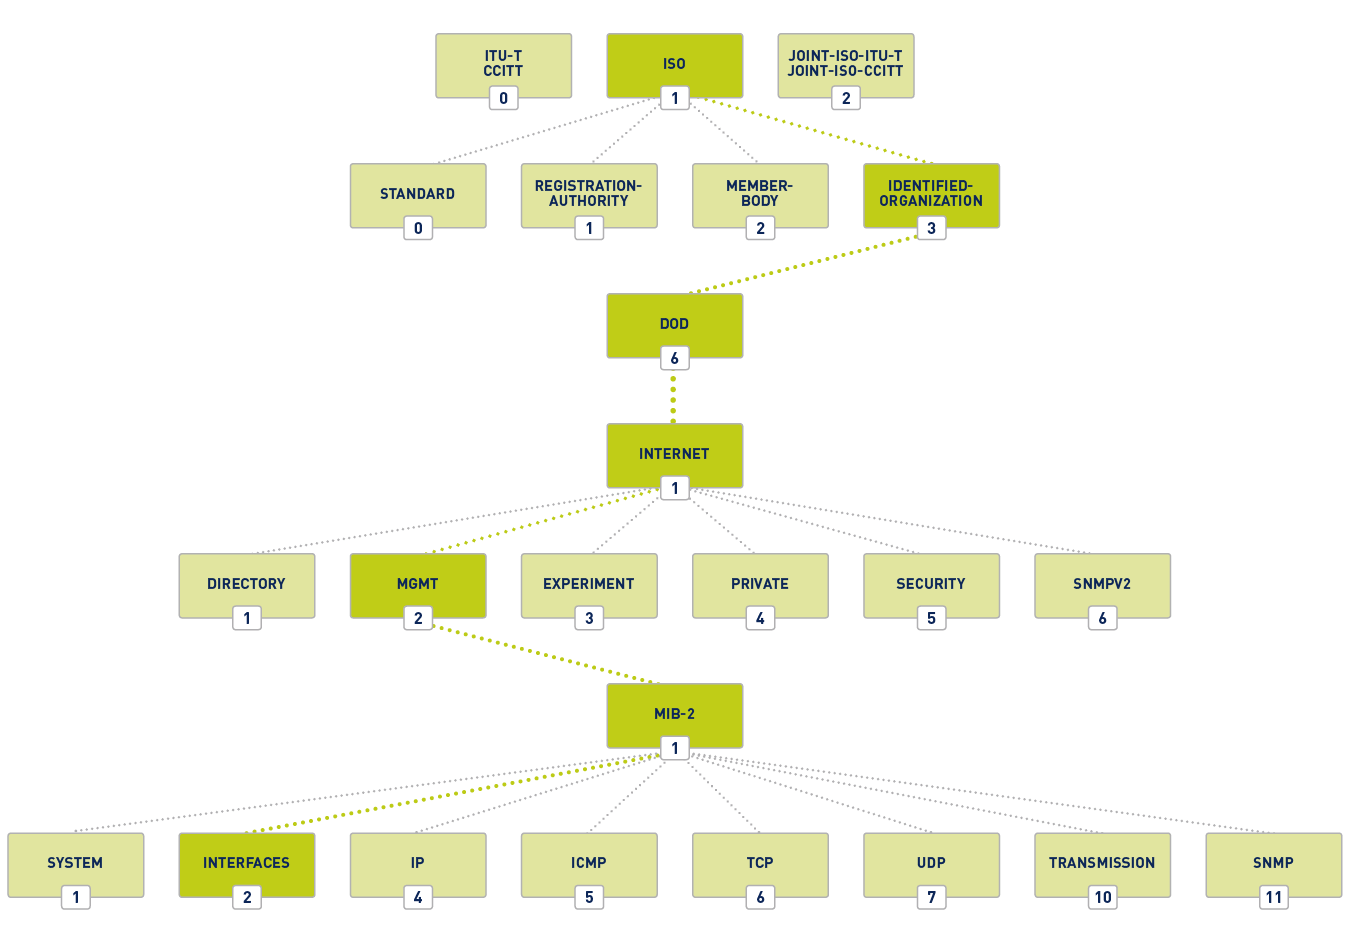
\includegraphics[ width=0.8\textwidth ]{pictures/OID-tree.png}
\end{figure}


\subsection{Configuration}

\subsubsection{SNMPv2}

\begin{enumerate}
\item (Required) Configure the community string and access level (read-only or read-write).

\begin{verbatim}
R1(config)# snmp-server community batonaug ro
\end{verbatim}

\item (Optional) Restrict SNMP access to NMS hosts (SNMP managers) using ACL. Step 1 and 2 can be done in one command.

\begin{verbatim}
R1(config)# snmp-server community batonaug ro SNMP_ACL
\end{verbatim}

\item (Optional) Enable traps on an SNMP agent. If no trap notification types are specified in this command, then all trap types are sent. Repeated use of this command is required if a particular subset of trap types is desired.

\begin{verbatim}
R1(config)# snmp-server enable traps
\end{verbatim}

\item (Optional) Specify the recipient of the SNMP trap operations.

\begin{verbatim}
R1(config)# snmp-server host 192.168.1.3 version 2c batonaug
\end{verbatim}

\item (Optional) Document the location of the SNMP server and the system contact.

\begin{verbatim}
R1(config)# snmp-server location NOC_SNMP_MANAGER
R1(config)# snmp-server contact Wayne World
\end{verbatim}

\end{enumerate}

\note To verify SNMP configuration, use any of the variations of the \texttt{show snmp} command.\\ 
\note Only the first step is required, the rest are optional.\\
\note By default, SNMP does not have any traps set. Without this command, SNMP managers must poll for all relevant information. 

\subsubsection{SNMPv3}

SNMPv3 provides three security features: Message integrity and authentication, Encryption, Access control. The following commands show an example of basic SNMPv3 configuration:

\begin{sexylisting}{SNMPv3 configuration}
R1(config)# snmp-server view SNMP-RO iso included                                    
R1(config)# snmp-server group ADMIN v3 priv read SNMP-RO access PERMIT-ADMIN         
R1(config)# snmp-server user BOB ADMIN v3 auth sha cisco12345 priv aes 128 cisco54321
\end{sexylisting}

In the above example, the first command creates an SNMP view \code{SNMP-RO} and include the entire \code{iso} tree from the MIB. The next command creates an SNMP group \code{ADMIN}, the set to version 3 (\verb|v3|) with authentication and encryption required. This command also gives read-only access to the view \code{SNMP-RO} to the group specified by the ACL called \code{PERMIT-ADMIN}. 

\section{NTP}

\subsection{System clock}

The software clock on a router or switch starts when the system boots and is the primary source of time for the system. It is important to synchronize the time across all devices on the network because all aspects of managing, securing, troubleshooting, and planning networks require accurate time-stamping. Typically, the date and time settings on a router or switch can be set using one of two methods: 

\begin{itemize}
\item Manually configure the date and time. For example, \verb|clock set 20:36:00 aug 30 2016|
\item Configure the NTP
\end{itemize}

\subsection{NTP operation}

NTP allows routers on the network to synchronize their time settings with an NTP server. It uses \textbf{UDP} port \textbf{123}. \\

NTP networks use a hierarchical system of time sources. Each level in this hierarchical system is called a \textbf{stratum}. The stratum level is defined as the number of hop counts from the authoritative time source (Figure \ref{NTP}). Smaller stratum numbers indicate that the server is closer to the authorized time source than larger stratum numbers. The max hop count is 15. Stratum 16, the lowest stratum level, indicates that a device is unsynchronized. 

\begin{figure}[hbtp]
\caption{NTP Stratum levels}\label{NTP}
\centering
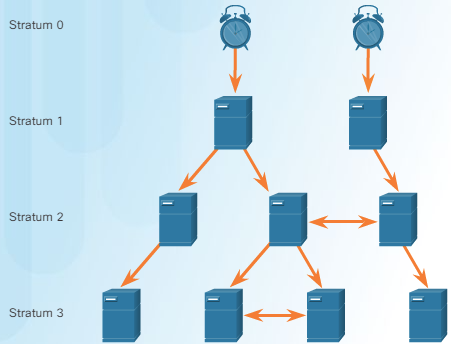
\includegraphics[ scale=0.6 ]{pictures/NTP.PNG}
\end{figure}

Stratum 0 is an NTP network that gets the time from authoritative time sources (represented by the clock in the figure \ref{NTP}). Stratum 1 are directly connected to the authoritative time sources. They act as the primary network time standard. The stratum 2 servers are connected to stratum 1 devices through network connections. Stratum 2 devices, such as NTP clients, synchronize their time using the NTP packets from stratum 1 servers. They can also act as servers for stratum 3 devices.

\subsection{Configure and Verify NTP}

To identify NTP server, use \code{ntp server <ip-addr>}.  Use \code{ntp update-calendar} to periodically update the hardware clock with the time learned from NTP. The following commands configure NTP authentication on R1 using key 1 and password NTPpa55. \\

To verify the system clock, use \code{show clock} command. To see if the device is synchronized with the NTP server, use \code{sh ip ntp ass} and \code{sh ntp status}.

\begin{sexylisting}{NTP authentication}
R1(config)# ntp server 192.168.1.5

R1(config)# ntp update-calendar

R1(config)# ntp authenticate
R1(config)# ntp trusted-key 1
R1(config)# ntp authentication-key 1 md5 NTPpa55

R1# sh ntp status
R1# sh ip ntp ass
R1# sh clock
\end{sexylisting}

\section{Cisco AutoSecure}

AutoSecure first makes recommendations for fixing security vulnerabilities and then modifies the security configuration of the router. It can lock down the management plane functions and the forwarding plane services and functions of a router. There are several management plane services and functions: firewall inspection, traffic filtering with ACLs, Secure password and login functions, Secure SSH access, Secure NTP, etc.\\

Use the \code{auto secure} command to enable the Cisco AutoSecure feature setup. In interactive mode, the router prompts with options to enable and disable services and other security features. This is the \emph{default} mode, but it can also be configured using the \code{auto secure full} command.\\

The non-interactive mode is configured with the \code{auto secure no-interact} command. This will automatically execute the Cisco AutoSecure feature with the recommended Cisco default settings. \\

When the AutoSecure command is initiated, a CLI wizard steps the administrator through the configuration of the device. User input is required. AutoSecure should be used when a router is initially being configured. It is not recommended on production routers.

\section{Control plane security}

\subsection{Routing protocol authentication}

\paragraph{Routing Protocol Spoofing:} Routing systems can be attacked by disrupting peer network routers, or by falsifying or spoofing the information carried within the routing protocols. Spoofing routing information may generally be used to cause systems to misinform (lie to) each other, cause a DoS attack, or cause traffic to follow a path it would not normally follow. 

\paragraph{OSPF MD5 Authentication:} OSPF supports routing protocol authentication using MD5  enabled globally for all interfaces or on a per interface basis.

\begin{sexylisting}{OSPF interface authentication}
R1(config)# interface s0/0/0
R1(config-if)# ip ospf message-digest-key 1 md5 cisco12345
R1(config-if)# ip ospf authentication message-digest
R1(config-if)# end
\end{sexylisting}

\begin{sexylisting}{OSPF area authentication}
R1(config)# router ospf 100
R1(config-router)# area 50 authentication message-digest
R1(config-router)# exit

R1(config)# interface s0/0/0
R1(config-if)# ip ospf message-digest-key 1 md5 cisco12345
R1(config-if)# end
\end{sexylisting}

\note The interface setting overrides the global setting. OSPF adjacency is lost until MD5 authentication is matched between two routers.\\

MD5 is now considered vulnerable to attacks. Therefore, the administrator should use SHA authentication as long as all of the router operating systems support OSPF SHA authentication. OSPF SHA authentication includes two major steps:

\begin{enumerate}
\item Specify an authentication key chain
\item Assign the authentication key to the desired interfaces 
\end{enumerate}

\begin{sexylisting}{OSPF SHA authentication}
Execute these commands for both routers

R1(config)# key chain HUY
R1(config-keychain)# key 1
R1(config-keychain-key)# key-string cisco12345
R1(config-keychain-key)# cryptographic-algorithm hmac-sha-256
R1(config-keychain-key)# exit

R1(config)# interface s0/0/0
R1(config-if)# ip ospf authentication key-chain HUY
\end{sexylisting}

\subsection{Control plane policing}

Routers must be able to distinguish between data plane, control plane, and management plane packets to treat each packet appropriately:

\begin{itemize}
\item \textbf{Data plane packets:} always have a transit destination IP address and can be handled by normal destination IP address-based forwarding processes.
\item \textbf{Control plane packets:} used for routing protocol (OSPF, EIGRP, BGP, etc.); sent to the router or network device
\item \textbf{Management plane packets:} used for management and reporting protocol (SSH, SNMP, NTP, etc.)
\end{itemize}

The vast majority of packets handled by network devices are data plane packets. They are handled by CEF. This forwarding method uses the control plane to pre-populate the FIB table. Subsequent packets that flow between same source and destination are forwarded by the data plane based on the information contained in the FIB.\\

\textbf{Control Plane Policing (CoPP)} is a Cisco IOS feature designed to allow administrators to manage the flow of traffic that is \emph{punted} to the route processor. It protects the route processor on network devices by treating route processor resources as a separate entity with its own interface. Unlike interface ACLs, no effort is wasted investigating data plane packets that will never reach the control plane.